\part{Introducción a la Metalurgia}


\section{Diferencia entre lo micro y macro}

Los conjuntos diseñados por ingenieros tienen una forma \textbf{geométrica} y un \textbf{material}. Ambas son propiedades macroscópicas. 

Sin embargo, lo que determina en gran parte las propiedades de una pieza es su \textbf{estructura} al nivel atómico (Å) y microscópico (micrómetros). Estas no son evidentes al ojo humano y se necesita de instrumentos y técnicas para poder detectar y caracterizar estas estructuras.

Un objetivo fundamental de la metalurgia física es tratar de relacionar los aspectos macroscópicos perceptibles con los aspectos microscópicos y submicroscópicos mediante métodos \textbf{netamente científicos}. La metalurgia física es una ciencia aplicada.

\section{Nociones de materiales}

\subsection{Grupos de Materiales}

\begin{description}
    \item[Metales] Materiales con enlaces metálicos
    \item[Polímeros] Sustancias inorgánicas con enlaces no metálicos
    \item[Polímeros] Matríz metálica, polimérica o cerámica con partículas o fibras poliméricas o cerámicas 
\end{description}


\subsection{Características de los metales}
Como clase de material, los metales son aquellos materiales cuyos átomos están unidos mediante un enlace metálico. Algunos materiales poseen enlaces no metálicos y son considerados metales porque su enlace metálico es el que prevalece, como es el caso para la mayoría de los metales estudiados.

\begin{itemize}
    \item Deformables plásticamente
    \item Fáciles de conformar y unir
    \item Alta tenacidad
    \item Alta resistencia mecánica
    \item Alta rigidez
    \item Bajo costo
    \item Alta conductividad eléctrica y térmica
    \item Fácilmente reciclables
    \item Baja resistencia a la corrosión
    \item Alta densidad
\end{itemize}

Los enlaces metálicos además son caracterizados por ser no-saturables (virtualmente no hay límite a la cantidad de electrones presentes) y no-direccionales.


\subsection{Aleaciones metálicas}

Se define como un material compuesto por varias clases de átomos (metálicos y/o no metálicos) unidos mediante un enlace principalmente metálico.

El \textbf{elemento base} de la aleación es el elemento químico mayoritario y siempre es de carácter metálico. Los \textbf{aleantes} son elementos cuya presencia se debe a una adición \textit{intencional} durante el proceso de fabricación de la aleación. Cumplen funciones específicas. En general hay un \textbf{aleante principal} que le otorga las características principales a la aleación y no tiene porque ser el de mayor proporción.

Los átomos que no fueron agregados intencionalmente sino que provienen de alguna/s de las materias primas usadas para la fabricación de la aleación (mineral, fundente, combustible, oxidante) y no han podido ser totalmente eliminados en el proceso de fabricación se llaman \textbf{residuales}. Se pueden categorizar en dos clases

\begin{description}
    \item[Residuales no nocivos] No tienen efectos negativos de importancia y pueden hasta mejorar alguna propiedad
    \item[Residuales nocivos o impurezas] Influyen negativamente en algunas propiedades de importancia para la aleación. Su reducción conlleva con un aumento del costo.  
\end{description}

\section{Unión entre átomos}

\begin{figure}
    \centering
    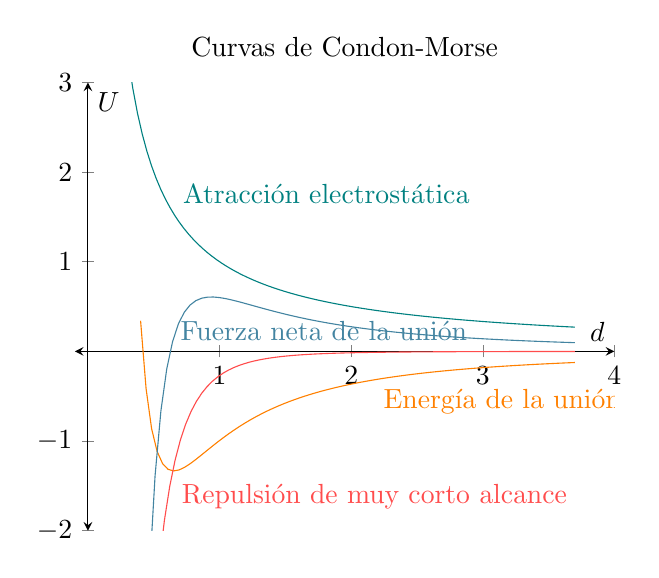
\begin{tikzpicture}[>=stealth]
    \begin{axis}[
        xmin=-.1,xmax=4,
        ymin=-2,ymax=3,
        axis x line=middle,
        axis y line=middle,
        axis line style=<->,
        xlabel={$d$},
        ylabel={$U$},
        title={Curvas de Condon-Morse},
        cycle list name=exotic,no marks
        ]
        \addplot expression[domain=.2:3.7,samples=100]{1/x} 
                    node[pos=0.5,anchor=south west]{Atracción electrostática}; 
        \addplot expression[domain=.4:3.7,samples=80]{(x-2*(x+.04)^2)/((x+.04)^4)}  
        node[pos=.7,anchor=north west]{Energía de la unión};
        \addplot expression[domain=.2:3.7,samples=80]{-(x-1.6*x^2)/((x)^4)}  
        node[pos=.96,anchor=south west]{Fuerza neta de la unión};
        \addplot expression[domain=.5:3.7,samples=80]{-1/(x+.3)^5}  node[pos=.3,anchor=north west]{Repulsión de muy corto alcance};
    \end{axis}
\end{tikzpicture}

\caption{Fuerzas que intervienen en una unión iónica. El punto donde la fuerza neta cruza el eje $x$ se denomina la distancia de equilibrio $d_0$ y es la distancia nominal entre átomos en un material. Este punto coincide con el mínimo de energía de la unión. Recordar que $F = - \frac{\textrm{d} U}{\textrm{d} x}$}.

\label{fig:curvas_condonmorse}

\end{figure}

\begin{itemize}
    \item El mínimo de energía ($U_0$) está relacionado con la temperatura de sublimación y fusión
    \item La pendiente de la curva de la fuerza neta sobre $d_0$ son proporcionales al módulo elástico del metal (se relaciona también con la curvatura de la energía sobre $d_0$ también)
    \item La asimetría de la curva de energía está relacionada con el coeficiente de dilatación del metal. Cuanto más empinada cerca de 0 y más chata alejándose de cero, más se dilata el material.
\end{itemize}



Al \textbf{aumentar} la energía de la unión, la distancia de equilibrio ($d_0$) disminuye (\textbf{disminuyendo la curvatura de la energía}), la curva de energía se vuelve \textbf{más simétrica}. En consecuencia puede decirse que, en términos generales, en los metales puros se cumple que a mayor punto de fusión es \textit{mayor} el módulo elástico y \textit{menor} el coeficiente de dilatación lineal.

\section{Estructura cristalina de metales}

En estado sólido los metales son cristalinos, es decir que los átomos ocupan posiciones ordenadas dentro de una estructura. Existen materiales metálicos sin ordenamiento en su estructura.

Existen materiales metálicos sin ordenamiento en su estructura (vidrios metálicos), pero son la excepción.

\begin{description}
    \item[Red cristalina] Red de puntos imaginarios que ocupan posiciones ordenadas en el espacio de modo que cada punto tiene idénticos alrededores
    \item[Motivo] Conjunto de átomos con una configuración determinada. Ocupa cada nodo de la red.
    \item[Estructura cristalina]  Red ordenada de puntos ubicándose en cada uno de ellos un mismo motivo constituido por átomos de metal
    \item[Parámetro de red] es la distancia entre átomos medida en las direcciones de los ejes principales de la celda de la red. Dependiendo de la configuración de la red (FCC/HCP/BCC) puede haber más de un parámetro. Suele ser del orden de unas décimas de nanómetro para metales.
\end{description}

\subsection{Características de estructuras cristalinas en metales}

\subsubsection{Estructura FCC}
Es una de las dos estructuras de máxima compacidad.
En general los FCC son metales de alta ductilidad y maleabilidad, baja tensión de fluencia, y alta tenacidad que además no presentan transición dúctil-frágil. 

\subsubsection{Estructura HCP}
Es una de las dos estructuras de máxima compacidad. Los HCP en general son metales menos dúctiles y más anisotrópicos que los FCC o BCC.


\subsubsection{Estructura BCC}
No posee planos de máxima compacidad. Los BCC poseen menor ductilidad y tenacidad que los FCC pero mayor tensión de fluencia. Presentan transición dúctil-frágil.

\subsection{Índices de Miller (incompleto)}

\subsection{Defectos cristalinos}

Las estructuras cristalinas reales no son perfectas. Todas presentan anomalías o apartamientos en el ordenamiento de sus átomos. Cualquier anomalía/apartamiento del orden perfecto se denomina un \textbf{defecto cristalino}.

Los defectos cristalinos son responsables por la diferencia entre la resistencia mecánica \textit{teórica} de los metales y la \textit{real}. A pesar de la reducción de resistencia teórica los defectos cristalinos tienen varios efectos positivos sobre las propiedades del metal (por ejemplo la capacidad de \textbf{deformar plásticamente} y capacidad de \textbf{endurecer} el metal)

Algunos de estos defectos son termodinámicamente estables (hacen descender la energía libre de Gibbs $G$) y por lo tanto el metal tiende a generarlos naturalmente durante el proceso de fabricación. Otros en cambio son inestables y se generan durante el procesamiento (def. plástica, solidificación) y son difícil de eliminar.

Todo defecto cristalino genera una \textbf{distorsión local en la red} a la cual está asociada una energía extra ya que los átomos vecinos no están en la posición de energía mínima ($d_0$ en las curvas de Condon-Morse, \ref{fig:curvas_condonmorse})

Esta distorsión genera un campo de tensiones elásticas alrededor del defecto. En consecuencia los defectos pueden interactuar entre sí atrayéndose o repeliéndose. 

\subsubsection{Defectos puntuales}
Hay tres tipos de defectos puntuales:

\begin{description}
    \item[Átomo sustitucional] Son átomos cuyo tamaño es lo suficientemente grande como para ocupar un lugar de la red. Si son de menor tamaño al aleante principal entonces genera un campo de compresión, atrayendo los átomos alrededor. Los sustitucionales de mayor tamaño al aleante principal generan un campo de tracción.
    \item[Átomo intersticial] Son lo suficientemente pequeños como para ocupar el espacio entre los nodos de la red provocando un campo de tracción. La distorsión que generan es muy grande y por ende la cantidad admitida por una red es muy pequeña. 
    \item[Vacancia] La ausencia de un átomo en un nodo de la red se denomina vacancia. Son un defecto necesario para que ocurra la \textbf{difusión de átomos sustitucionales}.
\end{description}

\subsubsection{Influencia de átomos intersticiales y sustitucionales}
Los átomos intersticiales y los sustitucionales ambos aumentan la entalpía H pero también la entropía S. Por eso, para cada elemento y para estado termodinámico existe una concentración máxima del mismo que puede ser admitida en la red de un metal dado. A esta concentración máxima se denomina \textbf{solubilidad}.


Debido a que tanto los elementos sustitucionales como los intersticiales bajan la energía libre de cualquier metal siempre que no pasen el límite de solubilidad, es difícil y costosa la obtención de metales de alta pureza (aplicaciones con necesidad de alta conductividad térmica/eléctrica). Por la misma razón es difícil evitar la contaminación de dichos metales durante su procesamiento o uso.

Aún así, en la mayoría de las aplicaciones no se requiere metales de alta pureza sino aleaciones que generalmente tienen mejores propiedades. 

En general lo átomos sustitucionales 
\begin{itemize}
    \item Endurecen el metal
    \item Reducen la tenacidad
    \item Disminuyen conductividad térmica/eléctrica
\end{itemize}


\subsubsection{Dislocaciones}

Este tipo de defecto \textbf{no está en equilibrio termodinámico}. Cada dislocación tiene un \textbf{vector de Burger único}, que indica la dirección de viaje de la dislocación.
Hay tres tipos de dislocaciones

\begin{description}
    \item[Dislocación de borde] La presencia de un plano de átomos incompleto produce este tipo de dislocación. El vector de Burger es perpendicular a la linea de dislocación.
    \item[Dislocación de hélice] Al querer hacer un circuito cerrado alrededor de la linea de dislocación se produce un desplazamiento que recuerda el paso de un tornillo/hélice. Su distorsión ocasionada genera una tensión local de corte.  El vector de Burger es paralelo a la linea de dislocación.
    \item[Dislocación mixta] Ocurre cuando la misma linea de dislocación de borde sigue para generar una dislocación de hélice (o vice-versa)
\end{description}

Las dislocaciones juegan un papel fundamental en la deformación plástica de los metales y en el endurecimiento que la misma produce, como veremos más adelante.

\subsubsection{Borde de grano}

Un borde de grano define el límite entre dos porciones de material con la misma estructura cristalina y composición pero de \textbf{diferente orientación}. No es lo mismo que una interfase.

\begin{description}
    \item[Monocristal] Es un material metálico con una única orientación de su red cristalina. En cualquier zona de ese material siempre se encuentra que la red cristalina está orientada de la misma forma.
    \item[Policristal] Material metálico en el qué existen zonas con diferente orientación de la red cristalina. Cada uno de estos sectores se denomina \textbf{grano del policristal} y tiene una orientación única de la red. \textit{La casi totalidad de materiales metálicos usados en la ingeniería son policristales debido al proceso de solidificación que favorece la formación de granos.}
\end{description}

El borde de grano es un defecto superficial que en general

\begin{itemize}
    \item Endurece el metal
    \item Hace descender la temperatura de transición dúctil-frágil
    \item Facilita la segregación. Zona de concentración preferencial de ciertas impurezas debido a la alta energía de un borde de grano
    \item Sitios preferenciales de transformación de fase. Muy relacionado a tratamientos térmicos
\end{itemize}

es por esto que la \textbf{reducción del tamaño de grano} es uno de los objetivos fundamentales en muchas aplicaciones de los metales.

Existen también los \textbf{bordes de subgranos}, llamado también borde de pequeño ángulo debido a que la desorientación entre los dos granos no supera los $1.5^\circ$. Está asociado a la formación de una pared de dislocaciones sobre el borde de grano para bajar la energía libre cuando no se puede eliminar dislocaciones.


\subsubsection{Superficie libre}

Los átomos ubicados en la superficie libre de un cristal poseen mayor energía que los del interior debido a que no poseen átomos de la red enfrentados a ellos y que compensen la acción de los átomos del interior del cristal.


\subsubsection{Interfases}

Una \textbf{interfase} separa dos fases diferentes, a diferencia de un borde de grano que separa la misma fase. Las dos fases pueden diferenciarse en \textbf{composición química} y/o \textbf{estructura cristalina} (no es lo mismo que \textit{orientación} cristalina).

La gran mayoría de los metales poseen varias fases y aún en pequeñas proporciones, ciertas fases pueden tener gran influencia en las propiedades del metal.

Tipos de interfases:

\begin{description}
	\item[Interfase coherente] Cuando existe continuidad de los planos cristalinos entre ambas fases
	\item[Interfase semi-coherente] Cuando existe continuidad entre algunos planos cristalinos entre ambas fases
	\item[Interfase incoherente] No hay continuidad alguna de planos cristalinos entre ambas fases  
\end{description}







